\section{Introduction} \label{intro}

High-throughput single-cell technologies have improved the resolution at which biological processes can be studied. A key component of such studies is differential abundance (DA) analysis, which aims to identify features that differ between experimental conditions.
However, the majority of established DA single-cell methods primarily detect changes in mean abundance and thus overlook other, biologically very informative, differences in distributions, such as changes in variance, skewness, modality, etc., limiting the advantages of single-cell over bulk analyses. This limiting focus stems from their origin in bulk omics workflows, where analyses beyond the mean are typically not feasible due to the limited number of available samples. Single-cell datasets, however, provide expression measurements for hundreds to thousands of individual cells, making it possible, and likely necessary, to assess changes in the full distribution of expression values.\\
%Restricting inference to mean-level changes risks overlooking more complex, yet biologically informative, differences in distributions, such as changes in variance, skewness, modality ...\\
Indeed, the importance of distribution changes is nicely illustrated in the SCP data from Leduc et al. \cite{leduc}, which compares melanoma cells with monocytes. Figure \ref{fig:examples} visualizes the density of three illustrative preprocessed proteins.

\begin{figure}[H]
    \centering
    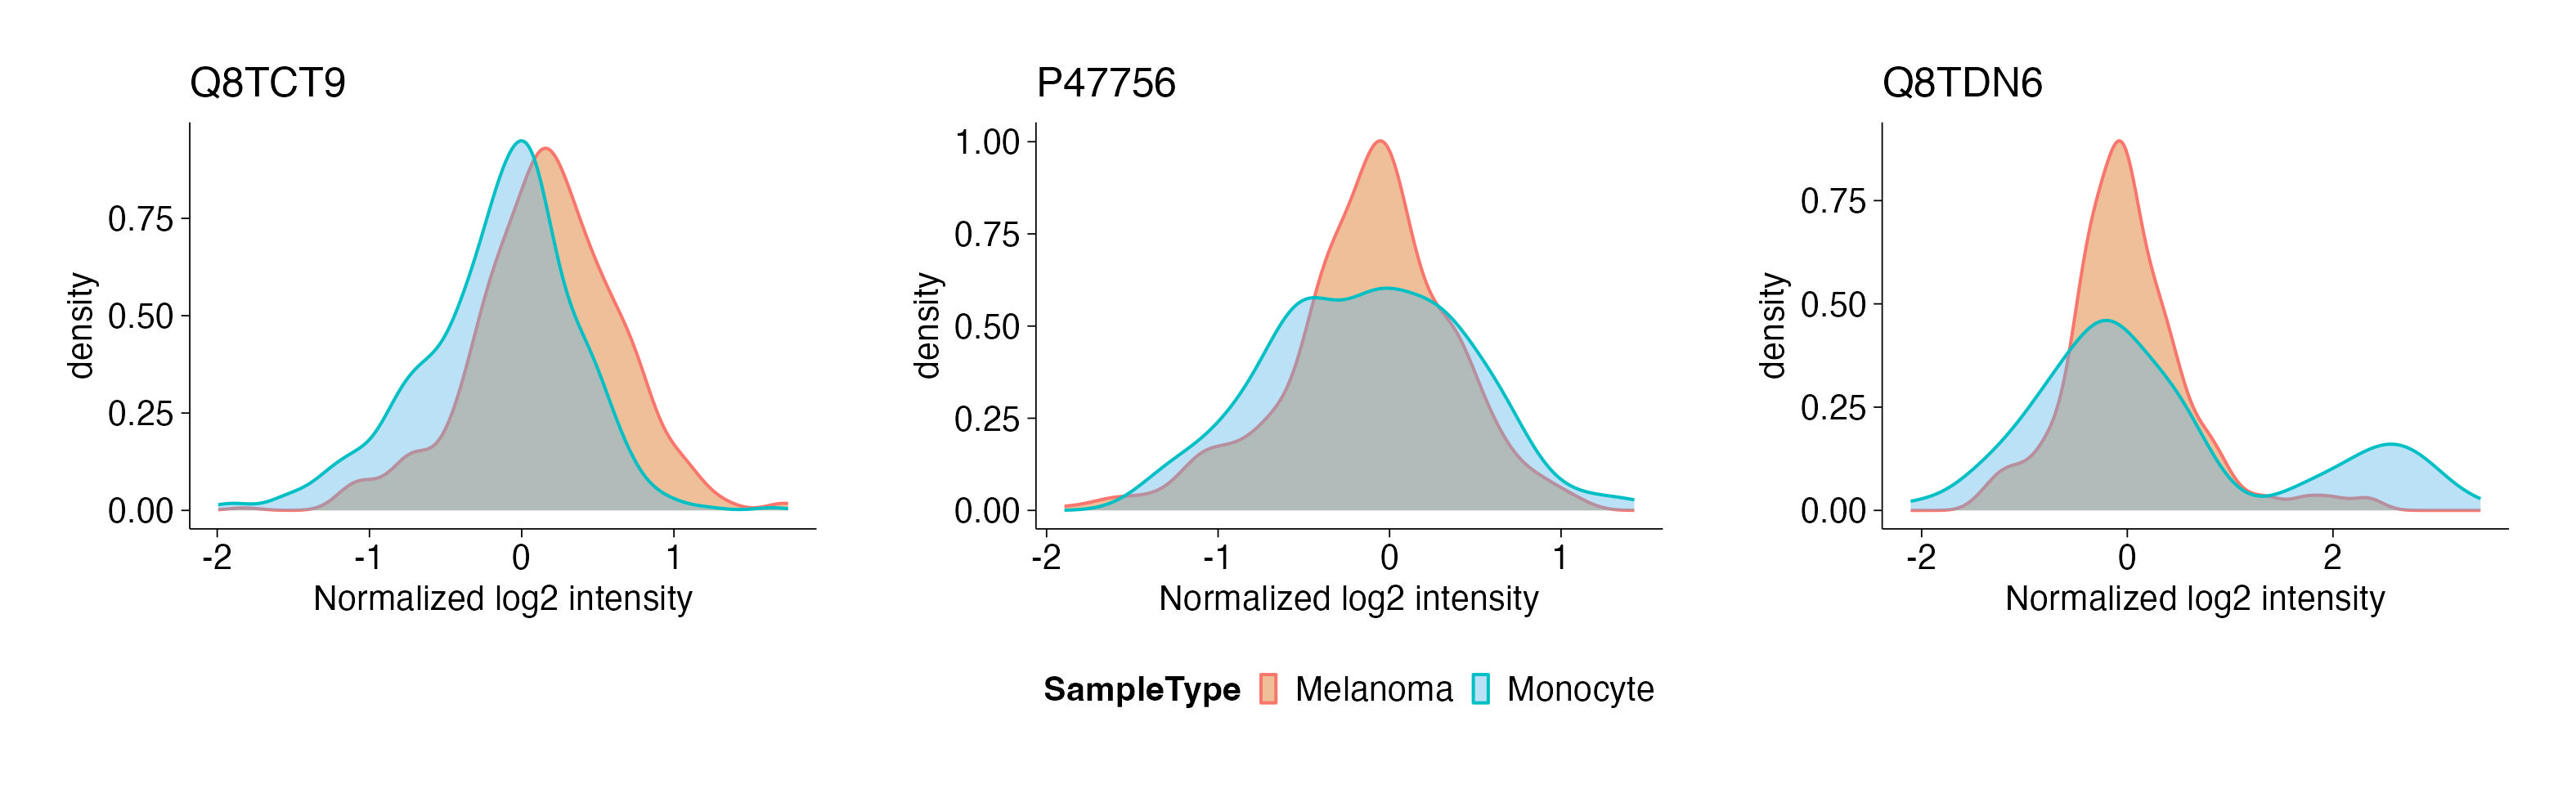
\includegraphics[width=\linewidth]{figs/fig1.jpg}
    \caption{\textbf{Motivating examples of distributional heterogeneity in single-cell proteomics} Density distributions of three proteins from the Leduc single-cell proteomics dataset, comparing melanoma cells (red) and monocytes (blue). The x-axis shows the normalized log2 protein intensity (log2-transformed, median-centered intensities; see Data in Methods), and the protein accession is given above each panel. The left panel (Q8TCT9) illustrates a conventional mean shift between cell types, which is the type of difference that standard DA methods are designed to detect. The middle panel (P47756) shows a difference in variance (Note that there is also a clear difference in kurtosis). The right panel (Q8TDN6) reveals the emergence of a distinct subpopulation in one cell type, visible as a secondary mode. The latter examples reflect differences in shape rather than mean. These are biologically informative yet systematically missed by conventional differential abundance (DA) approaches. They motivate the need for differential distribution (DD) methods capable of detecting the full spectrum of distributional differences in single-cell data.
}
    \label{fig:examples}
\end{figure}

Conventional DA analysis methods are designed to pick up mean shifts, as seen in the left panel in Figure \ref{fig:examples}, but lack power to prioritize proteins for which the distribution between cell populations mainly differs in shape, as seen in the middle and right panels in Figure \ref{fig:examples}.
%This illustrates a fundamental limitation of mean-based approaches: whether or not a distributional difference is deemed significant depends entirely on its impact on the mean.
These changes in shape may reflect underlying biological processes that remain undetected with conventional DA methods. For example, the increased
spread of the abundance values observed in the middle panel may indicate a heterogeneous cellular response, whereas the pattern in the right panel may reflect the emergence of a novel cell state in a subset of cells.
To infer such nuanced but relevant effects, more flexible approaches are required, which are referred to as differential distribution (DD) methods.
\\
\\
Several approaches to perform such DD analysis on single cell data already exist, most notably \texttt{BASiCS} \cite{basics}, \texttt{scDD} \cite{scdd} and \texttt{distinct} \cite{distinct}. However, these methods were developed specifically for single-cell RNA-seq data and have been neither tested on nor tailored for proteomics applications. Moreover, they cannot handle large proportions of missing values, a key problem in SCP datasets, and lack interpretability on how the distributions differ. The latter greatly limits the utility of the assessment, as the nature of the difference is an important element in hypothesizing about the possible causes.\\
Additionally, each approach has methodological limitations: \texttt{BASiCS} is restricted to testing for differences in mean and variance, \texttt{scDD} can only handle count data, and \texttt{distinct} can only be used for two-group comparisons.

Therefore we here present \texttt{gamdid}: a novel statistical framework for DD analysis. \texttt{gamdid} is capable of detecting any form of distributional difference between experimental conditions and provides an interpretable visualization of these effects. Importantly, \texttt{gamdid} also allows users to localize and visualize the specific regions that are differentially distributed, providing a direct link between statistical inference and visualization.\\
By building on the flexible framework of generalized additive models (GAMs), \texttt{gamdid} thus extends well beyond traditional mean-based comparisons while remaining intuitive and highly interpretable.



